% answers.tex —— 2010 年·普通高等学校招生考试·安徽卷·理科 · 参考答案与详细解析片段
% 由 tools/generate_projects.py 依来源总账自 2010/2010_数学真题_安徽理_试题.md + 2010/2010_数学真题_安徽理_解析正文.md + 2010/2010_数学真题_安徽理_答案要点.md 生成，勿手改（改源 MD 后重跑）

\begin{gktip}
固定候选 PDF 仅含题面，无答案页；以下解析与结论均由本库独立推导（非官方答案），并按 600 dpi 原页复核题面。原页未印分值，不补。
\end{gktip}

\begin{answer}
\gksolhead{1}{}

\textbf{题目}：

$\mathrm i$ 是虚数单位，$\dfrac{\mathrm i}{\sqrt3+3\mathrm i}=$（　）

（A）$\dfrac14-\dfrac{\sqrt3}{12}\mathrm i$

（B）$\dfrac14+\dfrac{\sqrt3}{12}\mathrm i$

（C）$\dfrac12+\dfrac{\sqrt3}{6}\mathrm i$

（D）$\dfrac12-\dfrac{\sqrt3}{6}\mathrm i$

\Needspace{4\baselineskip}
\textbf{解析}

\Needspace{5\baselineskip}
分子分母同乘 $\sqrt3-3\mathrm i$：

\nopagebreak[4]
\[\frac{\mathrm i}{\sqrt3+3\mathrm i}
=\frac{\mathrm i(\sqrt3-3\mathrm i)}{(\sqrt3)^2+3^2}
=\frac{3+\sqrt3\mathrm i}{12}
=\frac14+\frac{\sqrt3}{12}\mathrm i.\]

故选 B。

\gkanswer{答案：B。}

\end{answer}
\begin{answer}
\gksolhead{2}{}

\textbf{题目}：

若集合 $A=\left\{x\middle|\log_{\frac12}x\geqslant\dfrac12\right\}$，则 $\complement_{\mathbf R}A=$（　）

（A）$(-\infty,0]\cup\left(\dfrac{\sqrt2}2,+\infty\right)$

（B）$\left(\dfrac{\sqrt2}2,+\infty\right)$

（C）$(-\infty,0]\cup\left[\dfrac{\sqrt2}2,+\infty\right)$

（D）$\left[\dfrac{\sqrt2}2,+\infty\right)$

\Needspace{4\baselineskip}
\textbf{解析}

\Needspace{5\baselineskip}
因为 $y=\log_{\frac12}x$ 在 $(0,+\infty)$ 上单调递减，所以

\nopagebreak[4]
\[\log_{\frac12}x\geqslant\frac12=\log_{\frac12}\frac{\sqrt2}2
\iff 0<x\leqslant\frac{\sqrt2}2.\]

\Needspace{5\baselineskip}
故 $A=\left(0,\dfrac{\sqrt2}2\right]$，其补集为

\nopagebreak[4]
\[\complement_{\mathbf R}A=(-\infty,0]\cup\left(\frac{\sqrt2}2,+\infty\right).\]

故选 A。

\gkanswer{答案：A。}

\end{answer}
\begin{answer}
\gksolhead{3}{}

\textbf{题目}：

设向量 $\boldsymbol a=(1,0)$，$\boldsymbol b=\left(\dfrac12,\dfrac12\right)$，则下列结论中正确的是（　）

（A）$|\boldsymbol a|=|\boldsymbol b|$

（B）$\boldsymbol a\cdot\boldsymbol b=\dfrac{\sqrt2}2$

（C）$\boldsymbol a-\boldsymbol b$ 与 $\boldsymbol b$ 垂直

（D）$\boldsymbol a\parallel\boldsymbol b$

\Needspace{4\baselineskip}
\textbf{解析}

$|\boldsymbol a|=1$，$|\boldsymbol b|=\sqrt{\dfrac14+\dfrac14}=\dfrac{\sqrt2}2$，故 A 错；

\Needspace{5\baselineskip}
$\boldsymbol a\cdot\boldsymbol b=1\times\dfrac12+0\times\dfrac12=\dfrac12$，故 B 错；

\nopagebreak[4]
\[\boldsymbol a-\boldsymbol b=\left(\frac12,-\frac12\right),\qquad
(\boldsymbol a-\boldsymbol b)\cdot\boldsymbol b=\frac12\times\frac12-\frac12\times\frac12=0,\]

故 $\boldsymbol a-\boldsymbol b$ 与 $\boldsymbol b$ 垂直，C 对；

$\boldsymbol a$ 与 $\boldsymbol b$ 的坐标不成比例，D 错。

故选 C。

\gkanswer{答案：C。}

\end{answer}
\begin{answer}
\gksolhead{4}{}

\textbf{题目}：

若 $f(x)$ 是 $\mathbf R$ 上周期为 $5$ 的奇函数，且满足 $f(1)=1$，$f(2)=2$，则 $f(3)-f(4)=$（　）

（A）$-1$

（B）$1$

（C）$-2$

（D）$2$

\Needspace{4\baselineskip}
\textbf{解析}

\Needspace{5\baselineskip}
由 $f(x)$ 是周期为 $5$ 的奇函数，

\nopagebreak[4]
\[f(3)=f(3-5)=f(-2)=-f(2)=-2,\]

\nopagebreak[4]
\[f(4)=f(4-5)=f(-1)=-f(1)=-1.\]

故 $f(3)-f(4)=-2-(-1)=-1$。

故选 A。

\gkanswer{答案：A。}

\end{answer}
\begin{answer}
\gksolhead{5}{}

\textbf{题目}：

双曲线方程为 $x^2-2y^2=1$，则它的右焦点坐标为（　）

（A）$\left(\dfrac{\sqrt2}2,0\right)$

（B）$\left(\dfrac{\sqrt5}2,0\right)$

（C）$\left(\dfrac{\sqrt6}2,0\right)$

（D）$(\sqrt3,0)$

\Needspace{4\baselineskip}
\textbf{解析}

\Needspace{5\baselineskip}
把双曲线方程写成标准形式

\nopagebreak[4]
\[x^2-\frac{y^2}{\frac12}=1,\]

\Needspace{5\baselineskip}
则 $a^2=1$，$b^2=\dfrac12$，

\nopagebreak[4]
\[c^2=a^2+b^2=1+\frac12=\frac32,\qquad c=\frac{\sqrt6}2.\]

右焦点为 $\left(\dfrac{\sqrt6}2,0\right)$。

故选 C。

\gkanswer{答案：C。}

\end{answer}
\begin{answer}
\gksolhead{6}{}

\textbf{题目}：

设 $abc>0$，二次函数 $f(x)=ax^2+bx+c$ 的图象可能是（　）
\nopagebreak[4]
\begin{center}% 2010 年安徽卷理科第 6 题：四个二次函数图象选项（A）—（D）。
% 来源 PDF：普通高考/2010/2010安徽理.pdf，SHA-256 2760eb9e09374139a51303b0c2590746c74dfef7fed99ac6b2eace305af646c5。
% 原页：第 1 页（A3 三栏）第 1 栏，书页码 569。
% 重绘依据：四幅均只示意开口方向、y 轴截距符号与对称轴位置，不标刻度：
%   (A) 开口向下、截距为负、顶点在 y 轴左侧；(B) 开口向下、截距为正、顶点在右侧；
%   (C) 开口向上、截距为正、顶点在右侧；(D) 开口向上、截距为负、顶点在右侧。
\begin{tikzpicture}[semithick, scale=1.15, every node/.style={inner sep=1.2pt, font=\small}]
  % (A)
  \begin{scope}[shift={(0,0)}]
    \draw[-stealth] (-1.75,0) -- (0.75,0) node[right] {$x$};
    \draw[-stealth] (0,-0.95) -- (0,0.65) node[above] {$y$};
    \draw[thick,domain=-1.55:0.10,samples=80] plot (\x,{-0.8*(\x+0.9)^2+0.3});
    \node[below] at (-0.45,-1.35) {（A）};
  \end{scope}
  % (B)
  \begin{scope}[shift={(3.3,0)}]
    \draw[-stealth] (-0.55,0) -- (1.95,0) node[right] {$x$};
    \draw[-stealth] (0,-0.65) -- (0,1.05) node[above] {$y$};
    \draw[thick,domain=-0.45:1.85,samples=80] plot (\x,{-0.8*(\x-0.7)^2+0.9});
    \node[below] at (0.7,-1.35) {（B）};
  \end{scope}
  % (C)
  \begin{scope}[shift={(0,-3.1)}]
    \draw[-stealth] (-1.65,0) -- (1.65,0) node[right] {$x$};
    \draw[-stealth] (0,-0.75) -- (0,0.85) node[above] {$y$};
    \draw[thick,domain=-0.20:1.60,samples=80] plot (\x,{0.8*(\x-0.7)^2-0.2});
    \node[below] at (0.45,-1.35) {（C）};
  \end{scope}
  % (D)
  \begin{scope}[shift={(3.3,-3.1)}]
    \draw[-stealth] (-0.40,0) -- (1.95,0) node[right] {$x$};
    \draw[-stealth] (0,-0.80) -- (0,0.75) node[above] {$y$};
    \draw[thick,domain=-0.25:1.80,samples=80] plot (\x,{0.8*(\x-0.75)^2-0.6});
    \node[below] at (0.75,-1.35) {（D）};
  \end{scope}
\end{tikzpicture}
\end{center}
\nopagebreak[4]
\Needspace{4\baselineskip}
\textbf{解析}

由 $abc>0$ 可知 $a$，$b$，$c$ 全为正或一正两负，且 $a\neq0$。

（A）开口向下 $a<0$，与 $y$ 轴交于负半轴 $c<0$，故 $b>0$，对称轴 $x=-\dfrac b{2a}>0$，顶点应在 $y$ 轴右侧；图中顶点在左侧，矛盾。

（B）开口向下 $a<0$，与 $y$ 轴交于正半轴 $c>0$，故 $b<0$，对称轴 $x=-\dfrac b{2a}<0$，顶点应在 $y$ 轴左侧；图中顶点在右侧，矛盾。

（C）开口向上 $a>0$，与 $y$ 轴交于正半轴 $c>0$，故 $b>0$，对称轴 $x=-\dfrac b{2a}<0$，顶点应在 $y$ 轴左侧；图中顶点在右侧，矛盾。

（D）开口向上 $a>0$，与 $y$ 轴交于负半轴 $c<0$，故 $b<0$，对称轴 $x=-\dfrac b{2a}>0$，顶点在 $y$ 轴右侧，与图一致。

故选 D。

\gkanswer{答案：D。}

\end{answer}
\begin{answer}
\gksolhead{7}{}

\textbf{题目}：

设曲线 $C$ 的参数方程为 $\begin{cases}x=2+3\cos\theta,\\ y=-1+3\sin\theta\end{cases}$（$\theta$ 为参数），直线 $l$ 的方程为 $x-3y+2=0$，则曲线 $C$ 上到直线 $l$ 的距离为 $\dfrac{7\sqrt{10}}{10}$ 的点的个数为（　）

（A）$1$

（B）$2$

（C）$3$

（D）$4$

\Needspace{4\baselineskip}
\textbf{解析}

\Needspace{5\baselineskip}
曲线 $C$ 是圆心为 $(2,-1)$、半径为 $3$ 的圆。圆心到直线 $l:x-3y+2=0$ 的距离为

\nopagebreak[4]
\[d=\frac{|2-3\times(-1)+2|}{\sqrt{1+9}}
=\frac{7}{\sqrt{10}}=\frac{7\sqrt{10}}{10}.\]

这正是题设距离。过圆心作平行于 $l$ 的直线，它与圆交于 $2$ 个点；另一侧与 $l$ 距离同为 $\dfrac{7\sqrt{10}}{10}$ 的平行线到圆心距离为 $\dfrac{14\sqrt{10}}{10}>3$，与圆无公共点。

故满足条件的点有 $2$ 个。

故选 B。

\gkanswer{答案：B。}

\end{answer}
\begin{answer}
\gksolhead{8}{}

\textbf{题目}：

一个几何体的三视图如图，该几何体的表面积为（　）
\nopagebreak[4]
\begin{center}% 2010 年安徽卷理科第 8 题：几何体的三视图（正视图、侧视图、俯视图）。
% 来源 PDF：普通高考/2010/2010安徽理.pdf，SHA-256 2760eb9e09374139a51303b0c2590746c74dfef7fed99ac6b2eace305af646c5。
% 原页：第 1 页（A3 三栏）第 2 栏上部，书页码 569。
% 重绘依据：下部长方体 8×10×2；上部长方体 6×2×8，居中置于下部之上。
% 正视图宽 8、高 2，上部宽 6、两侧各 1；侧视图深 10、高 2，上部深 2、偏右 2；
% 俯视图 8×10，内框 6×2、距下边 2。
\begin{tikzpicture}[semithick, scale=0.38, every node/.style={inner sep=1.5pt, font=\small}]
  % 正视图
  \draw (0,0) rectangle (8,2);
  \draw (1,2) rectangle (7,10);
  \draw[<->] (0,10.45) -- node[above] {$1$} (1,10.45);
  \draw[<->] (1,10.45) -- node[above] {$6$} (7,10.45);
  \draw[<->] (7,10.45) -- node[above] {$1$} (8,10.45);
  \draw[<->] (-0.45,0) -- node[left] {$2$} (-0.45,2);
  \draw[<->] (-0.45,2) -- node[left] {$8$} (-0.45,10);

  % 侧视图
  \draw (11,0) rectangle (21,2);
  \draw (17,2) rectangle (19,10);
  \draw[<->] (11,10.45) -- node[above] {$6$} (17,10.45);
  \draw[<->] (17,10.45) -- node[above] {$2$} (19,10.45);
  \draw[<->] (19,10.45) -- node[above] {$2$} (21,10.45);
  \draw[<->] (21.45,0) -- node[right] {$2$} (21.45,2);
  \draw[<->] (21.45,2) -- node[right] {$8$} (21.45,10);

  % 俯视图
  \draw (4,-14) rectangle (12,-4);
  \draw (5,-12) rectangle (11,-10);
  \draw[<->] (12.45,-4) -- node[right] {$6$} (12.45,-10);
  \draw[<->] (12.45,-10) -- node[right] {$2$} (12.45,-12);
  \draw[<->] (12.45,-12) -- node[right] {$2$} (12.45,-14);
  \draw[<->] (4,-14.45) -- node[below] {$8$} (12,-14.45);

  \node at (4,-2.25) {正（主）视图};
  \node at (16,-2.25) {侧（左）视图};
  \node at (8,-16.2) {俯视图};
\end{tikzpicture}
\end{center}
\nopagebreak[4]
（A）$280$

（B）$292$

（C）$360$

（D）$372$

\Needspace{4\baselineskip}
\textbf{解析}

由三视图还原：下部是底面 $8\times10$、高 $2$ 的长方体；上部是底面 $6\times2$、高 $8$ 的长方体，置于下部长方体之上（正视图中上部宽 $6$、两侧各留 $1$，侧视图中上部深 $2$、宽 $8$ 的方向与俯视图对应）。

\Needspace{5\baselineskip}
下部表面积

\nopagebreak[4]
\[S_1=2(8\times10+8\times2+10\times2)=232,\]

\Needspace{5\baselineskip}
上部表面积

\nopagebreak[4]
\[S_2=2(6\times2+6\times8+2\times8)=152.\]

\Needspace{5\baselineskip}
两长方体接触面为 $6\times2=12$，在总面积中重复计算两次，故

\nopagebreak[4]
\[S=S_1+S_2-2\times12=232+152-24=360.\]

故选 C。

\gkanswer{答案：C。}

\end{answer}
\begin{answer}
\gksolhead{9}{}

\textbf{题目}：

动点 $A(x,y)$ 在圆 $x^2+y^2=1$ 上绕坐标原点沿逆时针方向匀速旋转，$12$ 秒旋转一周。已知时间 $t=0$ 时，点 $A$ 的坐标是 $\left(\dfrac12,\dfrac{\sqrt3}2\right)$，则当 $0\leqslant t\leqslant12$ 时，动点 $A$ 的纵坐标 $y$ 关于 $t$（单位：秒）的函数的单调递增区间是（　）

（A）$[0,1]$

（B）$[1,7]$

（C）$[7,12]$

（D）$[0,1]$ 和 $[7,12]$

\Needspace{4\baselineskip}
\textbf{解析}

\Needspace{5\baselineskip}
$t=0$ 时点 $A$ 的辐角为 $\dfrac\pi3$；$12$ 秒转一周，角速度为 $\dfrac{2\pi}{12}=\dfrac\pi6$。故

\nopagebreak[4]
\[y=\sin\left(\frac\pi3+\frac{\pi t}{6}\right).\]

\Needspace{5\baselineskip}
当 $0\leqslant t\leqslant12$ 时，辐角 $\theta=\dfrac\pi3+\dfrac{\pi t}{6}$ 从 $\dfrac\pi3$ 增加到 $\dfrac{13\pi}3$。正弦函数在 $\left[-\dfrac\pi2+2k\pi,\dfrac\pi2+2k\pi\right]$ 上递增，与 $\left[\dfrac\pi3,\dfrac{13\pi}3\right]$ 的交集为

\nopagebreak[4]
\[\left[\frac\pi3,\frac\pi2\right]\quad\text{\text{与}}\quad\left[\frac{3\pi}2,\frac{13\pi}3\right].\]

分别对应 $t\in[0,1]$ 与 $t\in[7,12]$。

故选 D。

\gkanswer{答案：D。}

\end{answer}
\begin{answer}
\gksolhead{10}{}

\textbf{题目}：

设 $\{a_n\}$ 是任意等比数列，它的前 $n$ 项和，前 $2n$ 项和与前 $3n$ 项和分别为 $X$，$Y$，$Z$，则下列等式中恒成立的是（　）

（A）$X+Z=2Y$

（B）$Y(Y-X)=Z(Z-X)$

（C）$Y^2=XZ$

（D）$Y(Y-X)=X(Z-X)$

\Needspace{4\baselineskip}
\textbf{解析}

设公比为 $q$。当 $q=1$ 时 $X=na_1$，$Y=2na_1$，$Z=3na_1$，逐项验证只有 D 成立。

\Needspace{5\baselineskip}
当 $q\neq1$ 时，

\nopagebreak[4]
\[Y-X=S_{2n}-S_n=q^nS_n=q^nX,\]

\nopagebreak[4]
\[Z-Y=S_{3n}-S_{2n}=q^{2n}S_n=q^{2n}X.\]

\Needspace{5\baselineskip}
于是

\nopagebreak[4]
\[(Y-X)^2=q^{2n}X^2=X\cdot q^{2n}X=X(Z-Y).\]

\Needspace{5\baselineskip}
展开得 $Y^2-2XY+X^2=XZ-XY$，即

\nopagebreak[4]
\[Y(Y-X)=X(Z-X).\]

故选 D。

\gkanswer{答案：D。}

\end{answer}
\begin{answer}
\gksolhead{11}{}

\textbf{题目}：

命题“对任何 $x\in\mathbf R$，$|x-2|+|x-4|>3$”的否定是$\underline{\qquad}$。

\Needspace{4\baselineskip}
\textbf{解析}

全称命题“对任何 $x\in\mathbf R$，$p(x)$”的否定是“存在 $x\in\mathbf R$，$\lnot p(x)$”，同时把“$>$”改为“$\leqslant$”。

故否定为：存在 $x\in\mathbf R$，使 $|x-2|+|x-4|\leqslant3$。

\gkanswer{答案：存在 $x\in\mathbf R$，使 $\lvert x-2\rvert+\lvert x-4\rvert\leqslant3$。}

\end{answer}
\begin{answer}
\gksolhead{12}{}

\textbf{题目}：

$\left(\dfrac{x}{\sqrt y}-\dfrac{y}{\sqrt x}\right)^6$ 的展开式中，$x^3$ 的系数等于$\underline{\qquad}$。

\Needspace{4\baselineskip}
\textbf{解析}

\Needspace{5\baselineskip}
设通项中取 $k$ 个 $-\dfrac{y}{\sqrt x}$，则

\nopagebreak[4]
\[T_{k+1}=\mathrm C_6^k\left(\frac{x}{\sqrt y}\right)^{6-k}\left(-\frac{y}{\sqrt x}\right)^k
=\mathrm C_6^k(-1)^k x^{6-\frac32k}y^{\frac32k-3}.\]

\Needspace{5\baselineskip}
令 $6-\dfrac32k=3$，得 $k=2$，此时 $y$ 的指数为 $0$。故 $x^3$ 的系数为

\nopagebreak[4]
\[\mathrm C_6^2(-1)^2=15.\]

\gkanswer{答案：$15$。}

\end{answer}
\begin{answer}
\gksolhead{13}{}

\textbf{题目}：

设 $x$，$y$ 满足约束条件 $\begin{cases}2x-y+2\geqslant0,\\ 8x-y-4\leqslant0,\\ x\geqslant0,\ y\geqslant0,\end{cases}$ 若目标函数 $z=abx+y$（$a>0$，$b>0$）的最大值为 $8$，则 $a+b$ 的最小值为$\underline{\qquad}$。

\Needspace{4\baselineskip}
\textbf{解析}

\Needspace{5\baselineskip}
约束条件对应可行域由直线 $y=2x+2$，$y=8x-4$ 与坐标轴围成，顶点为

\nopagebreak[4]
\[(0,0),\quad(0,2),\quad\left(\frac12,0\right),\quad(1,4).\]

\Needspace{5\baselineskip}
因为 $a>0$，$b>0$，所以 $z=abx+y$ 在 $(1,4)$ 取最大值，故

\nopagebreak[4]
\[ab+4=8,\qquad ab=4.\]

\Needspace{5\baselineskip}
由基本不等式

\nopagebreak[4]
\[a+b\geqslant2\sqrt{ab}=4,\]

当且仅当 $a=b=2$ 时取等号。故 $a+b$ 的最小值为 $4$。

\gkanswer{答案：$4$。}

\end{answer}
\begin{answer}
\gksolhead{14}{}

\textbf{题目}：

如图所示，程序框图（算法流程图）的输出值 $x=$ $\underline{\qquad}$。
\nopagebreak[4]
\begin{center}% 2010 年安徽卷理科第 14 题：算法流程图。
% 来源 PDF：普通高考/2010/2010安徽理.pdf，SHA-256 2760eb9e09374139a51303b0c2590746c74dfef7fed99ac6b2eace305af646c5。
% 原页：第 1 页（A3 三栏）第 3 栏上部，书页码 569。
% 重绘依据：开始 → x=1 → 判断「x 是奇数?」；是（右）→ x=x+1 → 回到判断前；
%   否（下）→ x=x+2 → 判断「x>8?」；否（右）→ 回到「x 是奇数?」前；是（下）→ 输出 x → 结束。
\begin{tikzpicture}[semithick, >=Stealth,
  every node/.style={inner sep=1.5pt, font=\small}]
  \node (start) [draw, rounded corners=4pt, minimum width=1.9cm, minimum height=0.55cm] at (0,0) {开始};
  \node (x1) [draw, minimum width=1.9cm, minimum height=0.55cm] at (0,-1.35) {$x=1$};
  \node (c1) [draw, diamond, aspect=2.1, minimum width=3.1cm,
    minimum height=1.15cm] at (0,-3.15) {$x$ 是奇数?};
  \node (p1) [draw, minimum width=2.5cm, minimum height=0.55cm] at (3.7,-3.15) {$x=x+1$};
  \node (p2) [draw, minimum width=2.5cm, minimum height=0.55cm] at (0,-4.85) {$x=x+2$};
  \node (c2) [draw, diamond, aspect=2.1, minimum width=3.1cm,
    minimum height=1.15cm] at (0,-6.65) {$x>8?$};
  \node (out) [draw, trapezium, trapezium left angle=72, trapezium right angle=108,
    minimum width=2.4cm, minimum height=0.55cm] at (0,-8.25) {输出 $x$};
  \node (end) [draw, rounded corners=4pt, minimum width=1.9cm, minimum height=0.55cm] at (0,-9.45) {结束};

  \draw[->] (start) -- (x1);
  \draw[->] (x1) -- (c1);
  \draw[->] (c1.east) -- node[above] {是} (p1.west);
  \draw[->] (c1.south) -- node[right] {否} (p2.north);
  \draw[->] (p2) -- (c2);
  \draw[->] (c2.south) -- node[right] {是} (out.north);
  \draw[->] (out) -- (end);
  % x=x+1 的回流
  \draw (p1.north) -- (3.7,-2.0) -- (0,-2.0);
  % x>8? 为否时的回流
  \draw (c2.east) -- node[above] {否} (5.2,-6.65) -- (5.2,-2.0) -- (0,-2.0);
  \draw[->] (0,-2.0) -- (c1.north);
\end{tikzpicture}
\end{center}
\nopagebreak[4]
\Needspace{4\baselineskip}
\textbf{解析}

初始 $x=1$。

\begin{itemize}
\item $x=1$ 为奇数，$x\leftarrow x+1=2$，$2\leqslant8$；
\item $x=2$ 为偶数，$x\leftarrow x+2=4$，$4\leqslant8$；
\item $x=4$ 为偶数，$x\leftarrow x+2=6$，$6\leqslant8$；
\item $x=6$ 为偶数，$x\leftarrow x+2=8$，$8\leqslant8$；
\item $x=8$ 为偶数，$x\leftarrow x+2=10$，此时 $10>8$，输出 $x=10$。
\end{itemize}

\gkanswer{答案：$10$。}

\end{answer}
\begin{answer}
\gksolhead{15}{}

\textbf{题目}：

甲罐中有 $5$ 个红球，$2$ 个白球和 $3$ 个黑球，乙罐中有 $4$ 个红球，$3$ 个白球和 $3$ 个黑球，先从甲罐中随机取出一球放入乙罐，分别以 $A_1$，$A_2$ 和 $A_3$ 表示由甲罐取出的球是红球，白球和黑球的事件；再从乙罐中随机取出一球，以 $B$ 表示由乙罐取出的球是红球的事件，则下列结论中正确的是$\underline{\qquad}$。（写出所有正确结论的编号）

① $P(B)=\dfrac25$；

② $P(B\mid A_1)=\dfrac5{11}$；

③ 事件 $B$ 与事件 $A_1$ 相互独立；

④ $A_1$，$A_2$，$A_3$ 是两两互斥的事件；

⑤ $P(B)$ 的值不能确定，因为它与 $A_1$，$A_2$，$A_3$ 中究竟哪一个发生有关。

\Needspace{4\baselineskip}
\textbf{解析}

先检验各结论。

\Needspace{5\baselineskip}
① 由全概率公式，

\nopagebreak[4]
\[P(B)=\frac5{10}\times\frac5{11}+\frac2{10}\times\frac4{11}+\frac3{10}\times\frac4{11}
=\frac{45}{110}=\frac9{22}\neq\frac25,\]

故①错。

\Needspace{5\baselineskip}
② 在 $A_1$ 发生的条件下，乙罐有 $5$ 个红球、共 $11$ 个球，故

\nopagebreak[4]
\[P(B\mid A_1)=\frac5{11},\]

②对。

③ 因为 $P(B\mid A_1)=\dfrac5{11}\neq\dfrac9{22}=P(B)$，所以 $B$ 与 $A_1$ 不独立，③错。

④ 从甲罐只取出一球，$A_1$，$A_2$，$A_3$ 不可能同时发生，任意两个也互斥，④对。

⑤ $P(B)$ 可由全概率公式确定，⑤错。

故正确结论为②④。

\gkanswer{答案：②④。}

\end{answer}
\begin{answer}
\gksolhead{16}{}

\textbf{题目}：

\Needspace{5\baselineskip}
设 $\triangle ABC$ 是锐角三角形，$a$，$b$，$c$ 分别是内角 $A$、$B$、$C$ 所对边长，并且

\nopagebreak[4]
\[\sin^2A=\sin\left(\frac\pi3+B\right)\sin\left(\frac\pi3-B\right)+\sin^2B.\]

（1）求角 $A$ 的值；

（2）若 $\overrightarrow{AB}\cdot\overrightarrow{AC}=12$，$a=2\sqrt7$，求 $b$，$c$（其中 $b<c$）。

\Needspace{4\baselineskip}
\textbf{解析}

\Needspace{5\baselineskip}
（1）由积化和差，

\nopagebreak[4]
\[\sin\left(\frac\pi3+B\right)\sin\left(\frac\pi3-B\right)
=\sin^2\frac\pi3\cos^2B-\cos^2\frac\pi3\sin^2B
=\frac34\cos^2B-\frac14\sin^2B.\]

\Needspace{5\baselineskip}
代入得

\nopagebreak[4]
\[\sin^2A=\frac34\cos^2B-\frac14\sin^2B+\sin^2B
=\frac34(\cos^2B+\sin^2B)=\frac34.\]

因为 $\triangle ABC$ 为锐角三角形，$A\in\left(0,\dfrac\pi2\right)$，故 $\sin A=\dfrac{\sqrt3}2$，$A=\dfrac\pi3$。

\Needspace{5\baselineskip}
（2）由 $\overrightarrow{AB}\cdot\overrightarrow{AC}=12$ 得

\nopagebreak[4]
\[bc\cos A=12,\qquad \frac12bc=12,\qquad bc=24.\]

\Needspace{5\baselineskip}
由余弦定理，

\nopagebreak[4]
\[a^2=b^2+c^2-2bc\cos A=b^2+c^2-bc=28,\]

\Needspace{5\baselineskip}
故 $b^2+c^2=52$，从而

\nopagebreak[4]
\[(b+c)^2=b^2+c^2+2bc=52+48=100,\]

\Needspace{5\baselineskip}
$b+c=10$。于是 $b$，$c$ 是方程 $t^2-10t+24=0$ 的两根，解得 $t=4$ 或 $6$。因 $b<c$，故

\nopagebreak[4]
\[b=4,\qquad c=6.\]

\gkanswer{答案：（1）$A=\dfrac\pi3$；（2）$b=4$，$c=6$。}

\end{answer}
\begin{answer}
\gksolhead{17}{}

\textbf{题目}：

设 $a$ 为实数，函数 $f(x)=\mathrm e^x-2x+2a$，$x\in\mathbf R$。

（1）求 $f(x)$ 的单调区间与极值；

（2）求证：当 $a>\ln2-1$ 且 $x>0$ 时，$\mathrm e^x>x^2-2ax+1$。

\Needspace{4\baselineskip}
\textbf{解析}

（1）$f'(x)=\mathrm e^x-2$。令 $f'(x)=0$ 得 $x=\ln2$。

当 $x<\ln2$ 时 $f'(x)<0$，$f(x)$ 单调递减；当 $x>\ln2$ 时 $f'(x)>0$，$f(x)$ 单调递增。

\Needspace{5\baselineskip}
故 $f(x)$ 在 $(-\infty,\ln2)$ 上递减，在 $(\ln2,+\infty)$ 上递增，在 $x=\ln2$ 处取得极小值

\nopagebreak[4]
\[f(\ln2)=\mathrm e^{\ln2}-2\ln2+2a=2a+2-2\ln2,\]

无极大值。

\Needspace{5\baselineskip}
（2）令

\nopagebreak[4]
\[g(x)=\mathrm e^x-x^2+2ax-1,\qquad x>0.\]

\Needspace{5\baselineskip}
则 $g(0)=0$，且

\nopagebreak[4]
\[g'(x)=\mathrm e^x-2x+2a,\qquad g''(x)=\mathrm e^x-2.\]

\Needspace{5\baselineskip}
$g''(x)$ 在 $x=\ln2$ 处取最小值 $0$，故 $g'(x)$ 在 $(0,+\infty)$ 上单调递增（$g''\geqslant0$），最小值为 $g'(\ln2)$：

\nopagebreak[4]
\[g'(\ln2)=2-2\ln2+2a=2(a-\ln2+1)>0.\]

\Needspace{5\baselineskip}
所以 $x>0$ 时 $g'(x)>0$，$g(x)$ 在 $(0,+\infty)$ 上单调递增，从而

\nopagebreak[4]
\[g(x)>g(0)=0,\]

即 $\mathrm e^x>x^2-2ax+1$。

\gkanswer{答案：（1）减区间 $(-\infty,\ln2)$，增区间 $(\ln2,+\infty)$，极小值 $2a+2-2\ln2$，无极大值；（2）证明见解析。}

\end{answer}
\begin{answer}
\gksolhead{18}{}

\textbf{题目}：

如图，在多面体 $ABCDEF$ 中，四边形 $ABCD$ 是正方形，$EF\parallel AB$，$EF\perp FB$，$AB=2EF$，$\angle BFC=90^\circ$，$BF=FC$，$H$ 为 $BC$ 的中点。

（1）求证：$FH\parallel$ 平面 $EDB$；

（2）求证：$AC\perp$ 平面 $EDB$；

（3）求二面角 $B-DE-C$ 的大小。
\nopagebreak[4]
\begin{center}% 2010 年安徽卷理科第 18 题：多面体 ABCDEF。
% 来源 PDF：普通高考/2010/2010安徽理.pdf，SHA-256 2760eb9e09374139a51303b0c2590746c74dfef7fed99ac6b2eace305af646c5。
% 原页：第 2 页（A3 三栏）第 1 栏下部，书页码 570。
% 重绘依据：ABCD 为正方形，EF∥AB 且 EF=AB/2；F 在 C 上方、E 在 D 上方；
%   BF、CF、EF、ED、EA、AB、BC、AD 为实线；CD、AC、BD 为不可见棱，画虚线；H 为 BC 中点。
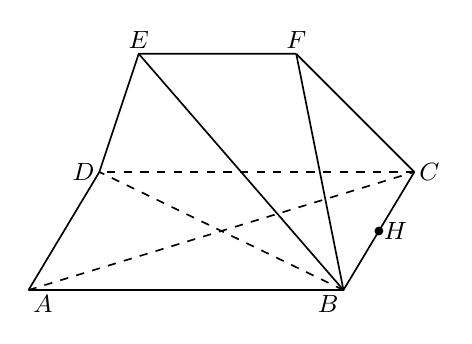
\begin{tikzpicture}[semithick, every node/.style={inner sep=1.5pt, font=\small}]
  \coordinate (A) at (0,0);
  \coordinate (B) at (4,0);
  \coordinate (C) at (4.9,1.5);
  \coordinate (D) at (0.9,1.5);
  \coordinate (E) at (1.4,3.0);
  \coordinate (F) at (3.4,3.0);
  \coordinate (H) at (4.45,0.75);

  \draw (A) -- (B) -- (C);
  \draw (A) -- (D) -- (E) -- (F) -- (E);
  \draw (F) -- (C);
  \draw (F) -- (B);
  \draw (E) -- (B);
  \draw[dashed] (C) -- (D);
  \draw[dashed] (A) -- (C);
  \draw[dashed] (B) -- (D);

  \fill (H) circle (1.6pt);
  \node[below right] at (A) {$A$};
  \node[below left] at (B) {$B$};
  \node[right] at (C) {$C$};
  \node[left] at (D) {$D$};
  \node[above] at (E) {$E$};
  \node[above] at (F) {$F$};
  \node[right] at (H) {$H$};
\end{tikzpicture}
\end{center}
\nopagebreak[4]
\Needspace{4\baselineskip}
\textbf{解析}

\Needspace{5\baselineskip}
以 $F$ 为原点，$FB$ 为 $x$ 轴，$FC$ 为 $y$ 轴，$FE$ 为 $z$ 轴建立空间直角坐标系。由 $BF=FC$，$\angle BFC=90^\circ$，$BC=2$，得 $BF=FC=\sqrt2$，故

\nopagebreak[4]
\[F(0,0,0),\quad B(\sqrt2,0,0),\quad C(0,\sqrt2,0).\]

\Needspace{5\baselineskip}
又 $EF\parallel AB$，$EF=1$，$AB=2$，且 $AB\perp$ 平面 $BFC$，故

\nopagebreak[4]
\[E(0,0,1),\quad A(\sqrt2,0,2),\quad D(0,\sqrt2,2).\]

\Needspace{5\baselineskip}
此时 $ABCD$ 是边长为 $2$ 的正方形。$H$ 为 $BC$ 中点，

\nopagebreak[4]
\[H\left(\frac{\sqrt2}2,\frac{\sqrt2}2,0\right).\]

（1）$\overrightarrow{FH}=\left(\dfrac{\sqrt2}2,\dfrac{\sqrt2}2,0\right)$。

\Needspace{5\baselineskip}
平面 $EDB$ 的法向量为

\nopagebreak[4]
\[\boldsymbol n=\overrightarrow{ED}\times\overrightarrow{EB}
=(0,\sqrt2,1)\times(\sqrt2,0,-1)
=(-\sqrt2,\sqrt2,-2).\]

\Needspace{5\baselineskip}
因为

\nopagebreak[4]
\[\overrightarrow{FH}\cdot\boldsymbol n=-\frac{\sqrt2}2\cdot\sqrt2+\frac{\sqrt2}2\cdot\sqrt2+0=0,\]

所以 $FH$ 平行于平面 $EDB$。又 $F\notin$ 平面 $EDB$，故 $FH\parallel$ 平面 $EDB$。

\Needspace{5\baselineskip}
（2）$\overrightarrow{AC}=C-A=(-\sqrt2,\sqrt2,-2)=\boldsymbol n$，故 $AC$ 与平面 $EDB$ 的法向量平行，即

\nopagebreak[4]
\[AC\perp\text{\text{平面} }EDB.\]

（3）平面 $CDE$ 经过 $C(0,\sqrt2,0)$，$D(0,\sqrt2,2)$，$E(0,0,1)$，三点 $x$ 坐标均为 $0$，故平面 $CDE$ 为 $x=0$，法向量可取 $\boldsymbol m=(1,0,0)$。

\Needspace{5\baselineskip}
设二面角 $B-DE-C$ 的大小为 $\theta$，则

\nopagebreak[4]
\[|\cos\theta|=\frac{|\boldsymbol n\cdot\boldsymbol m|}{|\boldsymbol n||\boldsymbol m|}
=\frac{\sqrt2}{\sqrt{2+2+4}}=\frac12,\]

故 $\theta=60^\circ$（由图知二面角为锐角）。

\gkanswer{答案：（1）证明；（2）证明；（3）$60^\circ$。}

\end{answer}
\begin{answer}
\gksolhead{19}{}

\textbf{题目}：

如图，已知椭圆 $E$ 经过点 $A(2,3)$，对称轴为坐标轴，焦点 $F_1$，$F_2$ 在 $x$ 轴上，离心率 $e=\dfrac12$。

（1）求椭圆 $E$ 的方程；

（2）求 $\angle F_1AF_2$ 的角平分线所在直线 $l$ 的方程；

（3）在椭圆 $E$ 上是否存在关于直线 $l$ 对称的相异两点？若存在，请找出；若不存在，说明理由。
\nopagebreak[4]
\begin{center}% 2010 年安徽卷理科第 19 题：椭圆 E、焦点 F1、F2、点 A 与角平分线 l。
% 来源 PDF：普通高考/2010/2010安徽理.pdf，SHA-256 2760eb9e09374139a51303b0c2590746c74dfef7fed99ac6b2eace305af646c5。
% 原页：第 2 页（A3 三栏）第 2 栏中部，书页码 570。
% 重绘依据：椭圆 x^2/16+y^2/12=1，F1(-2,0)、F2(2,0)，A(2,3)；
%   l 为 ∠F1AF2 的角平分线，方程 2x-y-1=0。
\begin{tikzpicture}[semithick, scale=0.95, every node/.style={inner sep=1.6pt, font=\small}]
  \draw[-stealth] (-4.6,0) -- (4.6,0) node[right] {$x$};
  \draw[-stealth] (0,-3.9) -- (0,4.1) node[above] {$y$};
  \draw[thick] (0,0) ellipse (4 and 3.464);
  \fill (-2,0) circle (1.6pt) node[below] {$F_1$};
  \fill (2,0) circle (1.6pt) node[below] {$F_2$};
  \fill (2,3) circle (1.6pt) node[above right] {$A$};
  \node[below left] at (0,0) {$O$};
  \draw[thick] (-0.25,-1.5) -- (2.15,3.3);
  \node[left] at (-0.25,-1.5) {$l$};
\end{tikzpicture}
\end{center}
\nopagebreak[4]
\Needspace{4\baselineskip}
\textbf{解析}

\Needspace{5\baselineskip}
（1）设椭圆方程为 $\dfrac{x^2}{a^2}+\dfrac{y^2}{b^2}=1$（$a>b>0$）。由 $e=\dfrac12$ 得 $c=\dfrac a2$，

\nopagebreak[4]
\[b^2=a^2-c^2=a^2-\frac{a^2}4=\frac34a^2.\]

\Needspace{5\baselineskip}
点 $A(2,3)$ 在椭圆上，

\nopagebreak[4]
\[\frac4{a^2}+\frac9{\frac34a^2}=1
\iff \frac4{a^2}+\frac{12}{a^2}=1
\iff a^2=16.\]

\Needspace{5\baselineskip}
故 $b^2=12$，椭圆 $E$ 的方程为

\nopagebreak[4]
\[\frac{x^2}{16}+\frac{y^2}{12}=1.\]

\Needspace{5\baselineskip}
（2）由（1）$c=2$，焦点为 $F_1(-2,0)$，$F_2(2,0)$。

\nopagebreak[4]
\[\overrightarrow{AF_1}=(-4,-3),\qquad \overrightarrow{AF_2}=(0,-3).\]

两方向的单位向量分别为 $\left(-\dfrac45,-\dfrac35\right)$ 与 $(0,-1)$，其和为 $\left(-\dfrac45,-\dfrac85\right)$，方向为 $(-1,-2)$，即角平分线的方向向量。

\Needspace{5\baselineskip}
故 $l$ 过 $A(2,3)$ 且方向为 $(-1,-2)$，方程为

\nopagebreak[4]
\[\frac{x-2}{-1}=\frac{y-3}{-2}
\iff 2x-y-1=0.\]

（3）假设存在关于 $l$ 对称的相异两点 $P$，$Q$。则 $PQ\perp l$，且 $PQ$ 的中点在 $l$ 上。

\Needspace{5\baselineskip}
$l$ 的斜率为 $2$，故 $PQ$ 的斜率为 $-\dfrac12$，可设 $PQ$ 所在直线为

\nopagebreak[4]
\[x+2y=m.\]

\Needspace{5\baselineskip}
设 $P(x_1,y_1)$，$Q(x_2,y_2)$，中点为 $M(x_0,y_0)$。对椭圆 $\dfrac{x^2}{16}+\dfrac{y^2}{12}=1$，斜率为 $-\dfrac12$ 的弦的中点满足

\nopagebreak[4]
\[\frac{x_0}{16}:\frac{y_0}{12}=1:2,\]

\Needspace{5\baselineskip}
即 $x_0=16\lambda$，$y_0=24\lambda$。又 $M\in l$，

\nopagebreak[4]
\[2x_0-y_0-1=0
\iff 32\lambda-24\lambda-1=0
\iff \lambda=\frac18.\]

故 $M=(2,3)=A$。

\Needspace{5\baselineskip}
于是 $PQ$ 是过 $A$ 且垂直于 $l$ 的直线，即 $x+2y=8$。但椭圆在 $A$ 处的切线方程为

\nopagebreak[4]
\[\frac{2x}{16}+\frac{3y}{12}=1
\iff x+2y=8,\]

它与椭圆仅切于点 $A$，不存在两个相异交点。矛盾。

故椭圆 $E$ 上不存在关于直线 $l$ 对称的相异两点。

\gkanswer{答案：（1）$\dfrac{x^2}{16}+\dfrac{y^2}{12}=1$；（2）$2x-y-1=0$；（3）不存在关于 $l$ 对称的相异两点。}

\end{answer}
\begin{answer}
\gksolhead{20}{}

\textbf{题目}：

\Needspace{5\baselineskip}
设数列 $a_1$，$a_2$，$\cdots$，$a_n$，$\cdots$ 中的每一项都不为 $0$。证明：$\{a_n\}$ 为等差数列的充分必要条件是：对任何 $n\in\mathbf N_+$，都有

\nopagebreak[4]
\[\frac1{a_1a_2}+\frac1{a_2a_3}+\cdots+\frac1{a_na_{n+1}}=\frac{n}{a_1a_{n+1}}.\]

\Needspace{4\baselineskip}
\textbf{解析}

设 $S_n=\dfrac1{a_1a_2}+\dfrac1{a_2a_3}+\cdots+\dfrac1{a_na_{n+1}}$。

\textbf{必要性}：若 $\{a_n\}$ 是公差为 $d$ 的等差数列，则 $a_{n+1}-a_n=d$。

\Needspace{5\baselineskip}
当 $d=0$ 时，$a_n=a_1$，

\nopagebreak[4]
\[S_n=\frac{n}{a_1^2}=\frac{n}{a_1a_{n+1}}.\]

\Needspace{5\baselineskip}
当 $d\neq0$ 时，

\nopagebreak[4]
\[\frac1{a_ka_{k+1}}=\frac1d\left(\frac1{a_k}-\frac1{a_{k+1}}\right),\]

\Needspace{5\baselineskip}
故

\nopagebreak[4]
\[S_n=\frac1d\left(\frac1{a_1}-\frac1{a_{n+1}}\right)
=\frac{a_{n+1}-a_1}{d\,a_1a_{n+1}}
=\frac{nd}{d\,a_1a_{n+1}}
=\frac{n}{a_1a_{n+1}}.\]

\Needspace{5\baselineskip}
\textbf{充分性}：已知对任意 $n\in\mathbf N_+$，

\nopagebreak[4]
\[\sum_{k=1}^n\frac1{a_ka_{k+1}}=\frac{n}{a_1a_{n+1}}.\]

\Needspace{5\baselineskip}
当 $n\geqslant2$ 时，用 $n$ 的等式减去 $n-1$ 的等式，得

\nopagebreak[4]
\[\frac1{a_na_{n+1}}
=\frac{n}{a_1a_{n+1}}-\frac{n-1}{a_1a_n}.\]

\Needspace{5\baselineskip}
两边同乘 $a_1a_na_{n+1}$，得

\nopagebreak[4]
\[a_1=na_n-(n-1)a_{n+1},\]

\Needspace{5\baselineskip}
即

\nopagebreak[4]
\[(n-1)(a_{n+1}-a_n)=a_n-a_1.\tag{$*$}\]

\Needspace{5\baselineskip}
记 $d_n=a_{n+1}-a_n$。由 $(*)$ 得

\nopagebreak[4]
\[(n-1)d_n=a_n-a_1.\]

\Needspace{5\baselineskip}
对 $n+1$ 同样有 $n d_{n+1}=a_{n+1}-a_1$。而

\nopagebreak[4]
\[a_{n+1}-a_1=(a_n-a_1)+(a_{n+1}-a_n)=(n-1)d_n+d_n=nd_n,\]

故 $n d_{n+1}=n d_n$，即 $d_{n+1}=d_n$（$n\geqslant2$）。又 $n=2$ 时 $d_2=a_2-a_1=d_1$，所以所有 $d_n$ 相等。

故 $\{a_n\}$ 为等差数列。充分性得证。

\gkanswer{答案：证明见解析。}

\end{answer}
\begin{answer}
\gksolhead{21}{}

\textbf{题目}：

品酒师需定期接受酒味鉴别功能测试，一般通常采用的测试方法如下：拿出 $n$ 瓶外观相同但品质不同的酒让其品尝，要求其按品质优劣为它们排序；经过一段时间，等其记忆淡忘之后，再让其品尝这 $n$ 瓶酒，并重新按品质优劣为它们排序，这称为一轮测试。根据一轮测试中的两次排序的偏离程度的高低为其评分。

现设 $n=4$，分别以 $a_1$，$a_2$，$a_3$，$a_4$ 表示第一次排序时被排为 $1,2,3,4$ 的四种酒在第二次排序时的序号，并令 $X=|1-a_1|+|2-a_2|+|3-a_3|+|4-a_4|$，则 $X$ 是对两次排序的偏离程度的一种描述。

（1）写出 $X$ 的可能值集合；

（2）假设 $a_1$，$a_2$，$a_3$，$a_4$ 等可能的为 $1,2,3,4$ 的各种排列，求 $X$ 的分布列；

（3）某品酒师在相继进行的三轮测试中，都有 $X\leqslant2$，

① 试按（2）中的结果，计算出现这种现象的概率（假定各轮测试相互独立）；

② 你认为该品酒师的酒味鉴别功能如何？说明理由。

\Needspace{4\baselineskip}
\textbf{解析}

\Needspace{5\baselineskip}
（1）$X=\sum\limits_{i=1}^4|i-a_i|$。由于

\nopagebreak[4]
\[X\equiv\sum_{i=1}^4(i-a_i)=0\pmod 2,\]

且 $0\leqslant X\leqslant|1-4|+|2-3|+|3-2|+|4-1|=8$，故 $X$ 只可能取 $0,2,4,6,8$。

这些值均可取到：恒等排列给 $X=0$；交换 $1,2$ 给 $X=2$；排列 $(2,1,4,3)$ 给 $X=4$；排列 $(2,3,4,1)$ 给 $X=6$；倒序排列 $(4,3,2,1)$ 给 $X=8$。

故 $X$ 的可能值集合为 $\{0,2,4,6,8\}$。

\Needspace{5\baselineskip}
（2）$24$ 种排列等可能。逐一枚举并按 $X$ 分类计数，得 $X=0,2,4,6,8$ 对应的排列数依次为 $1,3,7,9,4$。故分布列为

\nopagebreak[4]
\[P(X=0)=\frac1{24},\quad P(X=2)=\frac3{24}=\frac18,\quad P(X=4)=\frac7{24},\]

\nopagebreak[4]
\[P(X=6)=\frac9{24}=\frac38,\quad P(X=8)=\frac4{24}=\frac16.\]

\Needspace{5\baselineskip}
（3）① 由（2），

\nopagebreak[4]
\[P(X\leqslant2)=P(X=0)+P(X=2)=\frac1{24}+\frac3{24}=\frac16.\]

\Needspace{5\baselineskip}
三轮测试相互独立，故三轮都有 $X\leqslant2$ 的概率为

\nopagebreak[4]
\[\left(\frac16\right)^3=\frac1{216}.\]

② 若该品酒师完全没有鉴别能力，三轮都满足 $X\leqslant2$ 的概率仅为 $\dfrac1{216}\approx0.0046$，是一个小概率事件。现在这一事件发生了，说明更可能并非偶然，故可认为该品酒师有较强的酒味鉴别能力。

\gkanswer{答案：（1）$\{0,2,4,6,8\}$；（2）$P(X=0)=\dfrac1{24}$，$P(X=2)=\dfrac18$，$P(X=4)=\dfrac7{24}$，$P(X=6)=\dfrac38$，$P(X=8)=\dfrac16$；（3）① $\dfrac1{216}$，② 该品酒师有较强的酒味鉴别能力。}

\end{answer}